\documentclass[12pt]{article}
\usepackage[margin=1in]{geometry}
\usepackage{amssymb}
\usepackage{amsmath}
\usepackage{amsthm}
\usepackage{amsfonts}
\usepackage[shortlabels]{enumitem}
\usepackage{mathtools} 
\usepackage{amscd}        % For simple commutative diagrams
\usepackage{graphicx}
\usepackage{rotating}     % To rotate figures, tables, ...
\usepackage{color}
\usepackage{pdfpages}
\usepackage{blkarray, bigstrut, multirow}
\usepackage{hyperref}
\usepackage{wrapfig}


\begin{document}
\begin{titlepage}
    \begin{center}
        \vspace*{1cm}

        \textbf{Winning with Arclight Phoenix}

        \vspace{0.5cm}
        The way of the Bird

        \vspace{1.5cm}

        \textbf{Josh Mulloy}

        \vspace{0.8cm}

        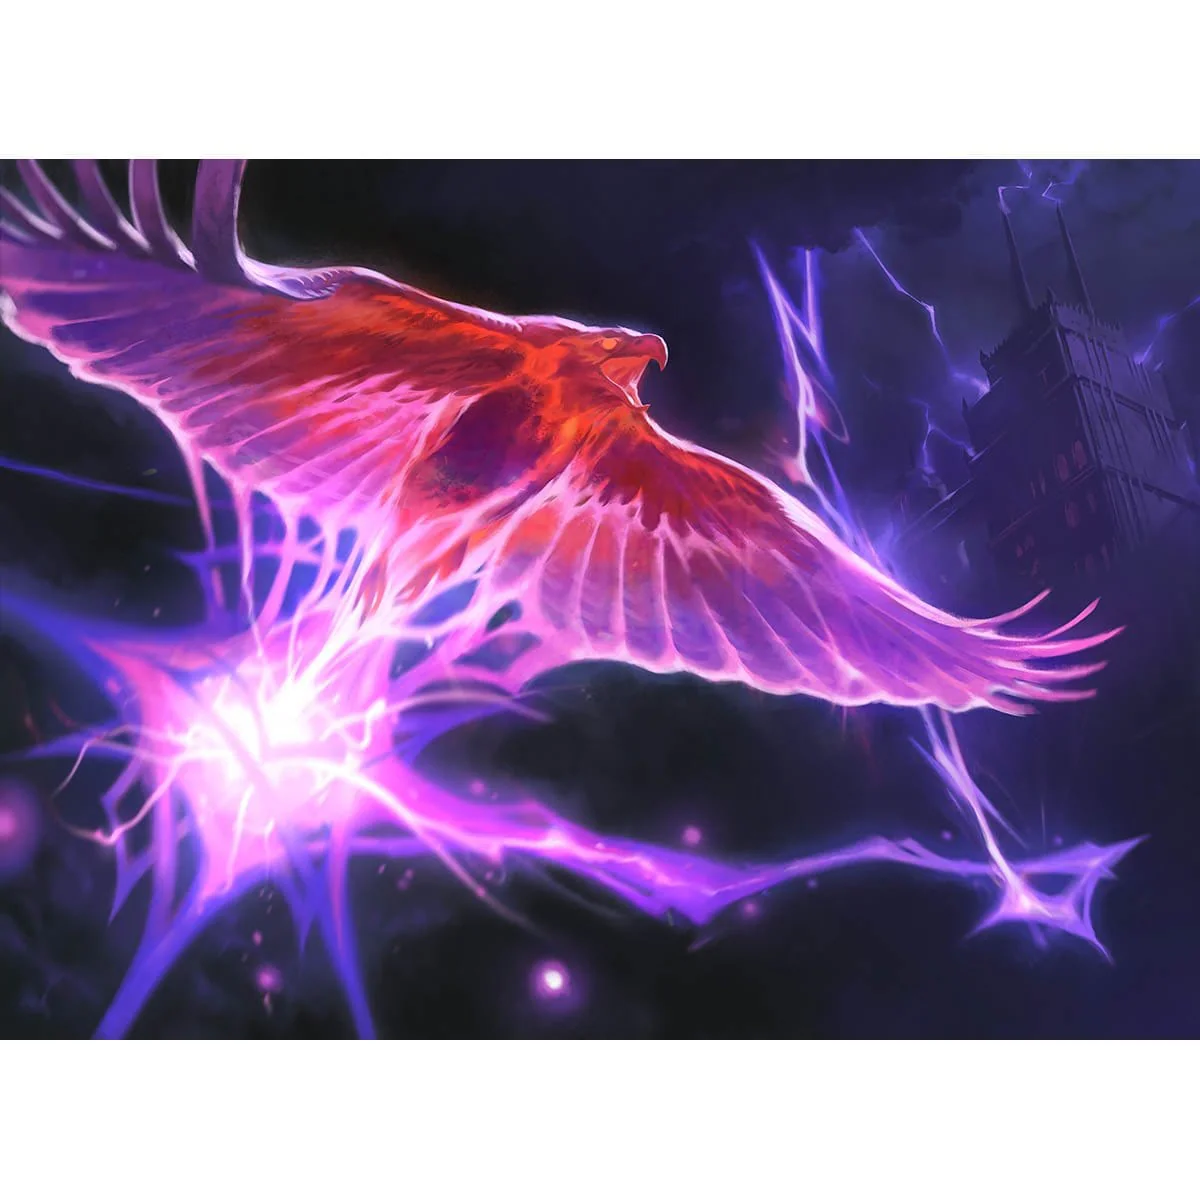
\includegraphics[width=0.7\textwidth]{arclight}

        \vfill

        A guide to playing arclight phoenix\\
        from one of the phoenix players of all time
    \end{center}
\end{titlepage}

\tableofcontents

\clearpage
\section{Current List}
\begin{center}
    \href{https://www.mtggoldfish.com/deck/6561022#online}{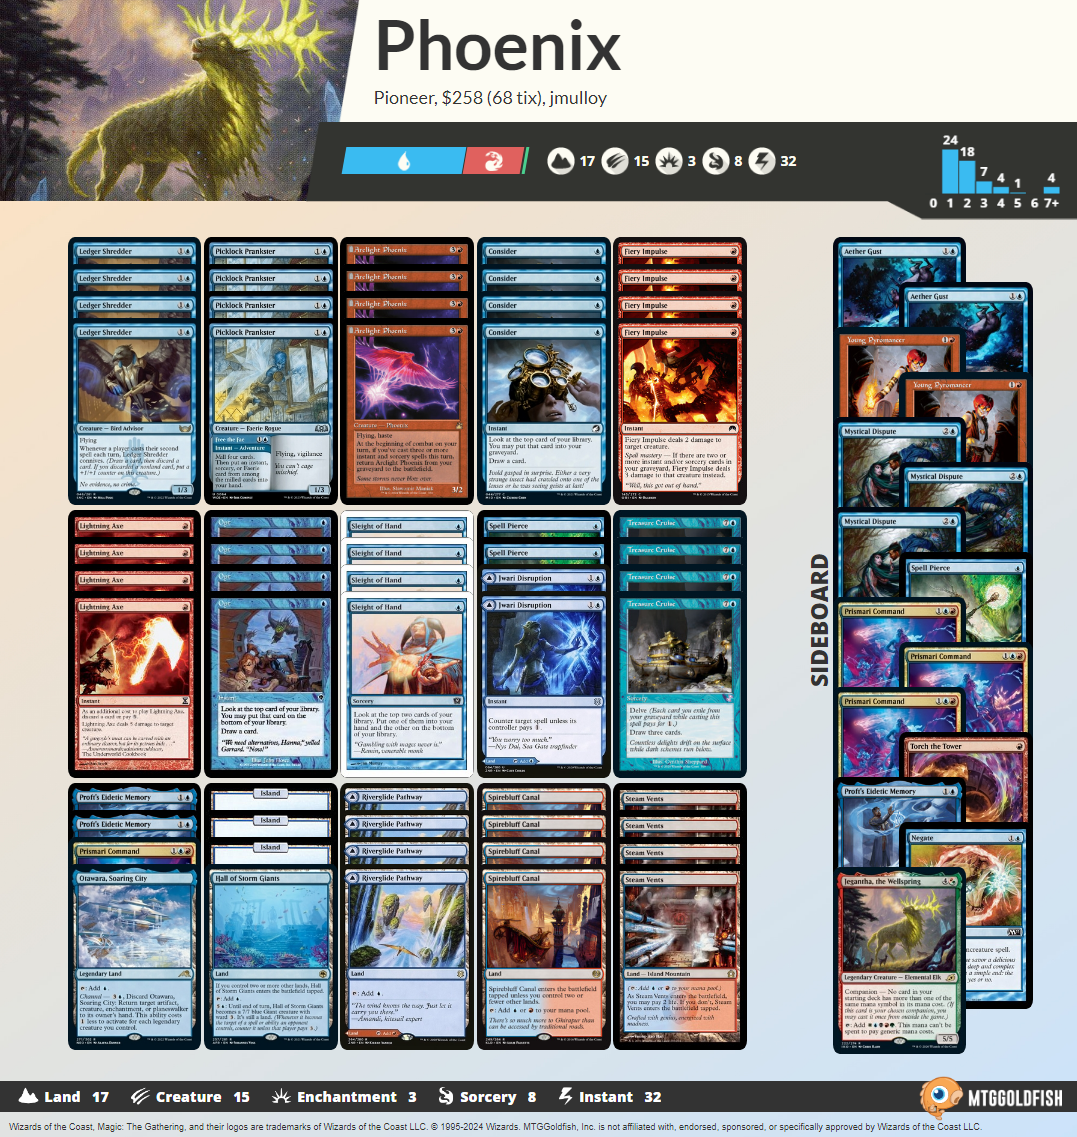
\includegraphics[width=1\textwidth]{decklist}}

    \href{https://www.mtggoldfish.com/deck/6561022}{https://www.mtggoldfish.com/deck/6561022}

    \vspace{0.5cm}

    \href{https://docs.google.com/spreadsheets/d/1DheUoGrQmpuwzbMDpPVJHcCrfe7UOyXSMSSkL8aXnv0/edit?usp=sharing}{Phoenix Matches (started tracking Aug 2024 [Challenge+ level]):}

    \href{https://docs.google.com/spreadsheets/d/1DheUoGrQmpuwzbMDpPVJHcCrfe7UOyXSMSSkL8aXnv0/edit?usp=sharing}{Spreadsheet Link}
\end{center}

\clearpage
\section{Why Phoenix?}
\subsection{Card Velocity}
Because phoenix plays 12 cantrips, 4 prankster, and 4 cruise, it is very easy to see most of your cards every game. This allows you to tune phoenix against basically any metagame, barring some pretty absurd things going on when phoenix is the clear best deck (like people registering waste not or lotus). Even when we are in one of these metas phoenix can still usually be tuned into a spot where we are fine into even these hate decks.

For example, with the newer prankster variants of phoenix we are able to play more spell pierce, depedning on the metagame. Some people even play a borrower in the main as a catch all that you can usually find when you need it. While I don't believe this to be better than just having Jegantha as a companion it speaks to how strong the ability to see so much of your deck is. This velocity is what makes the maindeck one ofs more interesting to me, things like maindeck primsari.

\subsection{Treasure Cruise}
I think a lot of people view phoenix as a deck that is just trying to put arclight phoenix into play as quickly as possible. While this is an admirable goal, it is not the main way that I play the deck. Often I would rather resolve a treasure crusie than put a single phoenix in play, and don't feel a strong urge to waste lightning axes because it will allow me to put phoenix into play.

As mentioned in the recent ban announcement, if phoenix manages to get another card banned in the format, its going to be cruise. The fact that we can chain cruise to go from empty handed to a full grip in a single turn for only two mana means that often even if an opponent manages to get a little ahead they will need to kill us fast.

\subsection{Low vs. High Resource Games}
Phoenix as a deck is really good at playing games where it always has things to be doing with its mana. I call these games \emph{high resource games}. They are the games where we cantrip a lot, resolve a few cruises, and maybe have a shredder that goes unanswered for a few turns. It is really hard for us to lose these kinds of games. The deck is just so capable of finding all the answers we need while also putting a ton of pressure on in these games that most decks have to somehow prevent us from getting into one. The low resource games are the ones where we are paying four mana for phoenix and 6 mana for lightning axe. They are the games where we don't find many cantrips and can't seem to find or maybe even cast a crusie.

Most of the games we lose are going to be games where we aren't able to get one of these high resource games going. This is what makes a lot of the hate so good into phoenix, but also what makes some of the hate less good than people think. Things like hearse, rip, and to a lesser extent leyline of the void are the main ways that decks try to keep us from creating high resource games. Leyline is specifically called out here because often we are able to turn a leyline game into a high resource game, or, if they don't have it in their opener, we can do enough to have a critical mass before they play it. The hate that is less good at stopping us in these spots are things like go blank, cling to dust, damping sphere, and grafdiggers cage. Just one of these cards isn't going to be enough to stop us, and in the case of cling, sphere, and cage I think these cards are just straight up bad into phoenix.

\subsection{It is Fun}
Phoenix is an interesting deck because you are able to see so many of your cards every game. You are going to have a ton of opporunities to make decisions, even if most of them don't matter, and that definitely makes it feel like you have more agency in the games than you do. For some reason I think this makes the game more fun for me. Furthermore, you just get to take a ton of game actions, and what are we playing magic for if not to take as many game actions as possible.

\vspace{0.4em}
\noindent I also just really like casting treasure cruise and attacking with 3/2s.

\clearpage
\section{The Details}
\subsection{Cantrip Sequencing}

\subsection{Playing Ledger Shredder}

\subsection{Graveyard Hate}

\subsection{Mulliganing}

\subsection{Paper Mechanics}

\clearpage
\section{Card Choices}
\subsection{Main Deck Cards}
\label{sec:mainchoices}
\textbf{Jegantha:}
Much better than I expected it to be. Really good as just a card that can be put in hand to pitch to axe/shredder. Also fine as a beater in the low resource games.

\vspace{0.4em}
\noindent \textbf{Proft's Eidetic Memory:}
Trespass plays pretty poorly with prankster, while this plays really well. Pretty sure this is just better in the mirror too. Definitely reduces our combo potential, making it a bit more important to chip in for damage when possible compared to the old phoenix lists, but you can still use this to kill people out of nowhere.

\vspace{0.4em}
\noindent \textbf{Cantrips:}
Seen lists playing 3 sleight, 4 opt, 4 consider. I feel quite strongly that you don't want to play less than the full 12. Sometimes we can trim a sleight during sideboarding, but this usually only comes up if we know our opponent has a lot of graveyard hate.

\vspace{0.4em}
\noindent \textbf{Fiery Impulse:}
Depending on the meta you can trim one of the fiery impulses for a pierce or even a proft or prismari. I don't think the meta is currently in one of those places but if phoenix becomes extremely popular we could be living in that world.

\vspace{0.4em}
\noindent \textbf{Spell Pierce:}
A nice catch all against basically every deck. It often comes out even if it has targets but I like it for game ones. Also nice as a one mana piece of interaction.

\vspace{0.4em}
\noindent \textbf{Prismari Command:}
Does everything we want in the low resource games, while also dealing with most of the actually good hate against us. All 4 modes come up often. An important part of casting crusie in low resource games, acting as a quadruple lotus petal a lot of the time. Basically, it is a good anti hate card that also just plays really well in the games before, after, and during the hate. I like the idea of having one in the main, but this maybe should just be a sideboard card.

\vspace{0.4em}
\noindent \textbf{Lands:}
The way I see it, phoenix lists have 4 flex slots for lands, usually choosing between 3rd island, hall of storm giants, jwari disruption, mountain, and stormcarved coast. I like jwari as something to bridge the gap to a turn 3 shredder that also gives us the ability to sometimes steal games by sniping something or making our opponent sequence weird. Hall is similar, where it is just there to shore up some games that we could be losing without it, specifically the low resource ones. I haven't felt a lot of pressure on red sources in my lists so I don't play an additional red source in mountain or stormcarved, but not playing them means you have to be a bit more careful deciding whether to put your pathways on red.

\vspace{0.4em}
\noindent \textbf{Trespass/Iteration:}
See Proft section above. I just don't think we really need this anymore, especially because it prevents us from playing Jegantha. It's possible we want it as people start trying to beat us as it's the best way to steal game one sometimes. It usually ends up coming out even in these spots though, making me think I'd rather just be all in on proft.

\vspace{0.4em}
\noindent \textbf{Artist's Talent:}
I haven't played with this yet, it might be good but I doubt it. I like the cards I play impacting the board, and we don't really need help discarding cards. I don't really see a world where this is better than shredder.

\vspace{0.4em}
\noindent \textbf{Torch the Tower:}
This card isn't better than impulse in basically any mu, including the mirror. I can't see myself ever playing one main.

\subsection{Sideboard Cards}
\label{sec:sbchoices}
\noindent \textbf{Prismari Command:}
See above.

\vspace{0.4em}
\noindent \textbf{Mystical Dispute:}
Best counterspell we can play.

\vspace{0.4em}
\noindent \textbf{Negate:}
I think we need some hard permission. It's possible that we can play more now that we are using picklock instead of pieces, although the matchups where we want this we plan to play as a tempo deck.

\vspace{0.4em}
\noindent \textbf{Spell Pierce:}
Better than second negate as it can answer a rest in peace on the draw. Depending on their list we might even want this against some RB mid opponents.

\vspace{0.4em}
\noindent \textbf{Aether Gust:}
The best card we can have against Mono Green. Also has big implications against Niv and dromoka out of lotus. Notably it is fine against red and can help us answer Kroxa out of RB. Basically just a really good catch all.

\vspace{0.4em}
\noindent \textbf{Proft's Eidetic Memory:}
This is our best card in the mirror, as well as against most of the creature decks. It also helps agaist people packing excessive graveyard hate.

\vspace{0.4em}
\noindent \textbf{Young Pyromancer:}
Helps us when we want to switch to a tempo deck against decks like lotus and UW control. Also has big impact against the creature decks without reach, like humans and GW company (not angels). I think people often overboard it against decks like RB that makes it look worse than it is. Some people play iconoclast in this spot, I think the fact that pyromancer can't be hit by mystical dispute is better than sometimes getting a creature off casting a proft.

\vspace{0.4em}
\noindent \textbf{Torch the Tower:}
I currently have one of these as a ninth one mana removal spell against aggro decks. I still don't like the card but I think it may be a necessary evil.

\vspace{0.4em}
\noindent \textbf{Crackling Drake:}
I have always found crackling drake to be very awkward but necessary. Now that we have profts as our big card against graveyard hate, as well as prismari to better answer hate, I think it is less needed. It is just super awkward that you tap out to play it and your opponent can often kill it and advance their board putting you way behind, although this is offset by them usually dying if you untap. I think we just no longer need it, especially because proft lets us have Jegantha post board in the matchups where it's best.

\vspace{0.4em}
\noindent \textbf{Thing in the Ice:}
A very good card against green and company decks (to the extent it can be good into skyclave). I don't think it's that good into basically anything else, with it being quite a bit worse than just another removal spell against mono red and mono white. The fact that the green decks can't slow down our graveyard plan as much anymore makes me want to play this much less, although it is quite good against angels if that makes a comeback.

\vspace{0.4em}
\noindent \textbf{Brotherhood's End:}
In the past we have used this card as an answer to artifact hate and trespasser out of RB mid. It's also fine as a wrath against the aggro decks, although it has diminishing returns against mono white and mono red. If the GW company decks become more popular it likely gets better but I'm unconvinced it will be better than something like Thing in the Ice that lets us keep Jegantha.

\vspace{0.4em}
\noindent \textbf{Anger of the Gods:}
Without Amalia in the format anymore this card is significantly worse than brotherhood's end.

\vspace{0.4em}
\noindent \textbf{Ashiok, Dream Render:}
Probably the best hate card we can play. It is quite good in the mirror, although weak to dispute and pierce, while also having good interactions against Lotus and Niv. Against the mirror I think it is better to be on the proft side than the Ashiok side, and against Lotus and Niv I would rather just be trying to tempo them out. The fact this turns off Jegantha is a bit less relevant as the matchups Ashiok is good aren't really the matchups where Jegantha is best. For now I think I'm going to leave Ashiok out but I could see wanting it.

\vspace{0.4em}
\noindent \textbf{Blue Sun's Twilight:}
This is my favorite sideboard card I've ever played in phoenix. It is a very clean answer to fable that also has some big implications in the Sheoldred and Kroxa fights aginst RB. Unforuntalely I don't think it does enough to warrant losing Jegantha in the fable matchups.

\vspace{0.4em}
\noindent \textbf{Behold the Multiverse:}
I am considering that this card could be good in the thoughtseize and the control matchups. I played it a while ago and always liked it but it is probably a lot worse now that we have prankster and aren't skipping turn two much. It does let us keep Jegantha which is neat.

\clearpage
\section{Matchups and Sideboarding}
Sideboarding spreadsheet: \href{https://docs.google.com/spreadsheets/d/1DheUoGrQmpuwzbMDpPVJHcCrfe7UOyXSMSSkL8aXnv0/edit?gid=1532833725}{link}
\subsection{Phoenix Mirror}
In all the games the early turns are all about ledger shredder. In game one you usually want to hold shredder until you can get it out of impulse range immediately without making it vulnerable. This makes it so that often you can't jam it on turn 2 on the draw and will need to try to wait to get a better opporunity. On the play you are more capable to just jam on turn 2. After that, if a shredder survives the game quickly becomes trying to get it to six toughness, although it will still be weak to two removal spells in game one.

\begin{wrapfigure}{r}{0.25\textwidth}
    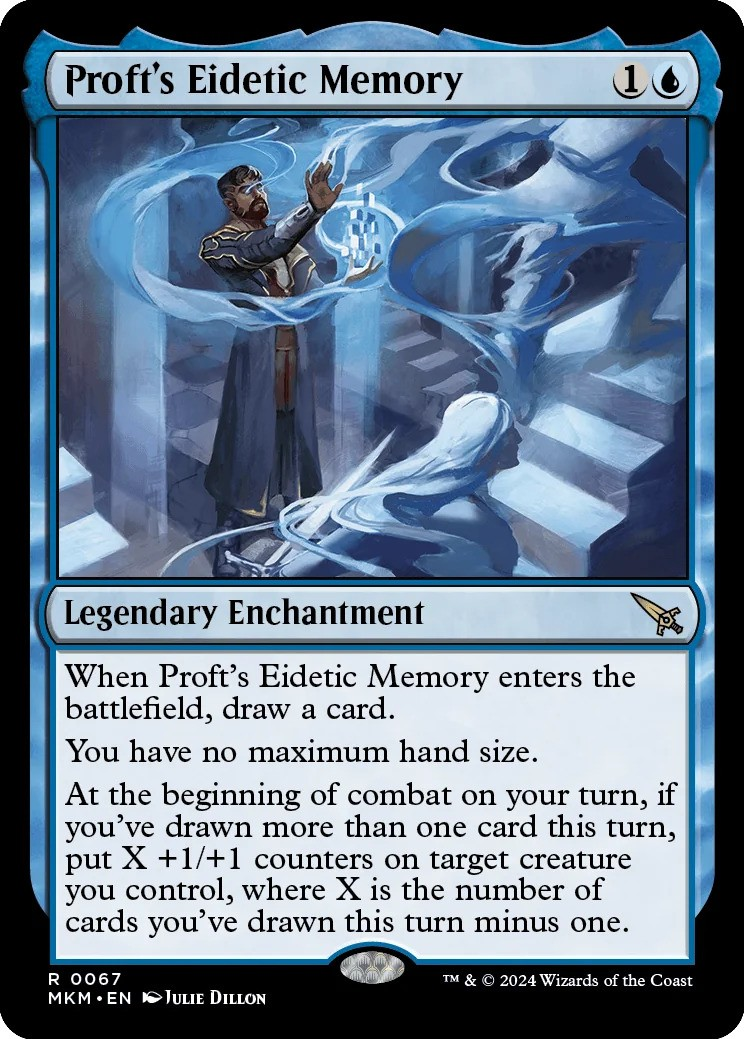
\includegraphics[width=0.9\linewidth]{Cards/proft.jpg}
\end{wrapfigure}

After that the game becomes more about proft, especially proft with prankster as a huge vigilance creature is just really hard to deal with. Because proft is so good you often hace to try to hold a way to remove the creature it targets, sometimes allowing them to trigger shredder. It's possible that proft is good enough to want to leave in fiery impulse post board, but its a dead card most of the time and I don't think enough people have more than two proft to start doing that. Proft is so good in the mirror that I put the third in the board specifically to go up to three.

Post board this matchup becomes a bit slower, with both players bringing in a lot of counterspells. One of the key interactions post board is trying to fight shredder with dispute as the cleanest answer to not give up a trigger. Often it comes up on turn 3 that someone wants to shredder with dispute or pierce backup, even in this situation dispute is good as it allows you to kill it with axe without wasting a mana or giving a trigger.

In the past some people had hearse for the matchup as graveyard hate but nowadays most people just have Ashiok if they have any hate. If they are on hearse we want some number of prismari, but hearse is really bad in the phoenix board so I wouldn't worry about it unless I've seen it. The best way to beat Ashiok is to counter it, but if you know that your hand is weak to it you can hold picklock to have a chance at cruising after an activation. Some people like alt threats like young pyromancer here, I generally find them quite underwhelming although it's possible they are fine now that we are planning to try to proft them and can overload their removal. In the past I found that negate wasn't very good because you usually have stuff to do with that extra mana. It's possible that if you know your opponent is on trespass then negate is worth it. It also might be better on the draw as a way to answer Ashiok when we are less likely to have a threat to attack it.

\begin{center}
    \begin{tabular}{|l|l|}
        \hline
        In             & Out        \\
        \hline
        1 Proft's      & 4 Impulse  \\
        3 Dispute      & 1 Prismari \\
        1 Spell Pierce &            \\
        \hline
    \end{tabular}
\end{center}

\subsection{RB Mid}
I think this matchup used to be very close and slightly favored for them but since we started playing picklock and proft I believe it has flipped and we are favored. In game one it is all about trying to stock a graveyard and cast treasure crusie. The main thing that we are trying to avoid happening in game one is getting our phoenixes hit by graveyard trespasser. They usually only have two so we don't have to be super worried about it but it is one of their best ways to steal the first game.

\begin{wrapfigure}{r}{0.25\textwidth}
    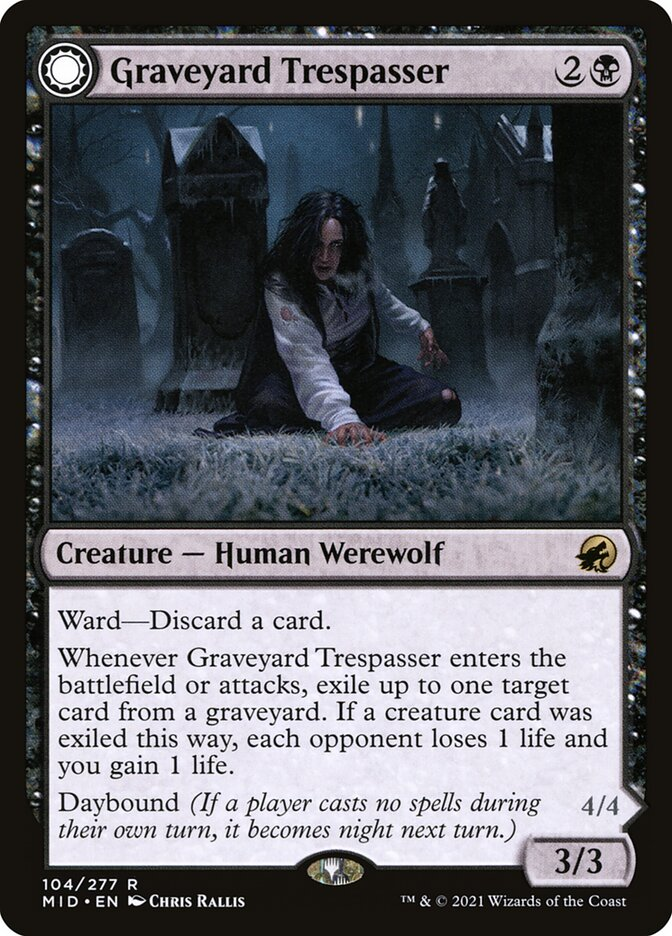
\includegraphics[width=0.9\linewidth]{Cards/trespasser.jpg}
\end{wrapfigure}

Because they are a thoughtseize deck our mulligans can get a bit looser, although I try to avoid going to crazy with this. You still want to spend as much of your mana as possible and get to a spot where you can draw cruise and cast it. Usually they are going to go after your pranksters with thoughtseize early and that can put us in weird spots where we have to spend a lot of mana on cruise.

Sheoldred is obviously very annoying for us when it sits in play for any number of turns. For this reason we usually want to be a bit stingy with our use of lightning axe when we have one, although this changes when we are using an axe as a third spell to bring back phoenixes. Usually we have to try to preserve our life total so that we are capable of digging for an axe even if we don't have one. The other big issue that they sometimes have is archfiend. Our answers to this one are less clean and so if we know they are playing it we sometimes have to try to hold two removal spells for it. Generally I try to be quite defensive with my early phoenixes so that I can prevent getting into spots where I have to spend removal spells that I want to spend on either of these cards.

Post board they are going to have some number of hearse and then a combination of Ashiok and go blank. Because of the amount of expensive noncreature stuff coming in, we sometimes want a pierce or two. The problem is that sometimes they don't have to play those or fable on curve, and then pierce ends up looking very bad. Generally I just like bringing in the prismari as a better removal spell than fiery impulse that also plays really nice into their bankbuster and hearse plans. Other cards you can consider are proft if you think they are light on removal and aether gust if you've seen Kroxa. Kroxa can becomes a really big problem so usually once I know they have one I'll bring in a single gust. It isn't worth it if you're just trying to use it to deal with fable.

The cards that we don't want are some of the removal spells. Even though they both have good targets the games we lose are usually the ones where we draw too many of them and aren't able to get the ball rolling. Generally I cut fiery impulse first then start looking at trimming some lightning axe, never going below three axe. In the past we have sometimes boarded out shredder, I no longer do this as I think that we are fine with it getting pushed since if it survives we usually just win the game easily. Usually their sideboard plan involves boarding out bonecrusher so we don't even have that many good targets for fiery impulse, although we usually want some for trespasser.

\begin{center}
    \begin{minipage}[t]{0.35\linewidth}
        \begin{tabular}[t]{|l|l|}
            \multicolumn{2}{c}{\textbf{Kroxa}} \\
            \hline
            In             & Out               \\
            \hline
            2 Impulse      & 3 Prismari        \\
            1 Axe          & 1 Gust            \\
            1 Spell Pierce &                   \\
            \hline
        \end{tabular}
    \end{minipage}
    \quad
    \begin{minipage}[t]{0.35\linewidth}
        \begin{tabular}[t]{|l|l|}
            \multicolumn{2}{c}{\textbf{No Kroxa}} \\
            \hline
            In        & Out                       \\
            \hline
            3 Impulse & 3 Prismari                \\
            \hline
        \end{tabular}
    \end{minipage}
\end{center}

\subsection{Mono Green}
This matchup used to be significantly more challenging when they had Karn into tormod's crypt. Now they don't have a whole lot of cards that matter. They are going to win the games where they have leyline plus early Nykthos, but usually we are going to be able to kill the things that matter and eventually take over with mutliple phoenixes or proft. The best way to win games in this matchup is to play a turn two ledger shredder.

\begin{wrapfigure}{r}{0.25\textwidth}
    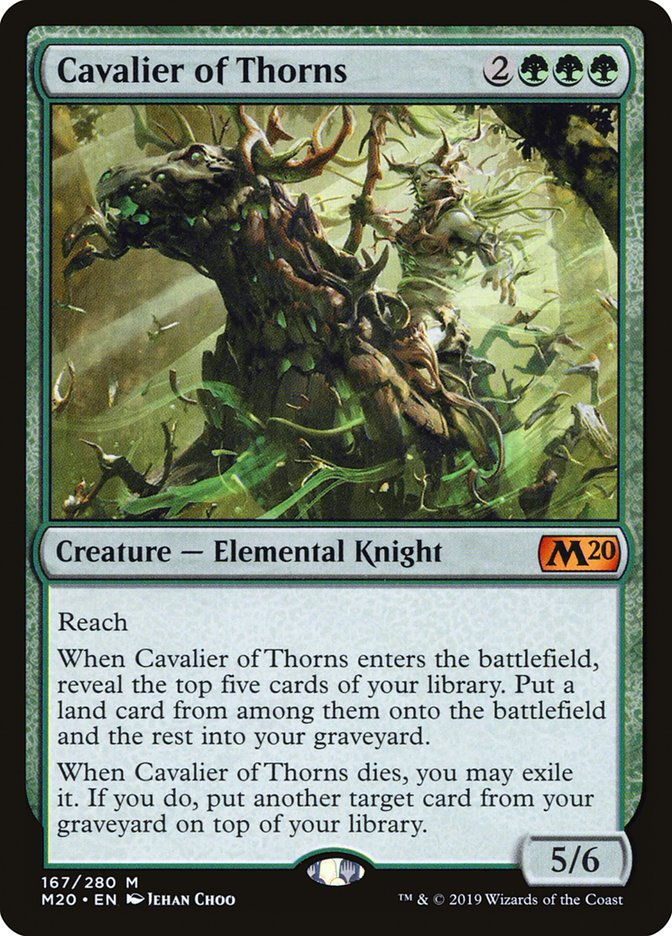
\includegraphics[width=0.9\linewidth]{Cards/cav.jpg}
\end{wrapfigure}

One of the cards that gives us the most trouble here is Cavalier. It blocks well and usually we can't kill it until the turn that we plan to kill our opponent as otherwise they get to draw the best card in their graveyard. The best way to beat it is to get a big shredder or picklock with proft and go over it, while also being able to block well. For this reason getting your creatures to 3/5 so they can block troll and 4/6 to block cav becomes very important. The main way they can win once you have a big creature that can block is by comboing and eventually giving a big board haste. To avoid this happening the best thing we can do is find a lightning axe and hold it up for as long as possible to kill oddity in response to it flipping. You do have to be a bit careful here because sometimes they can get to enough mana to activate the flip ability twice.

When sideboarding we get better ability to interact. Our lightning axes line up quite poorly, especially against turn one elf, so we want to trim them for so aether gust. Additionally, because our plan leans heavily on ledger shredder and proft we are able to trim a phoenix. Spell pierce also isn't very good, although it does have some implications against Kiora and wolfwillow. The extra proft comes in to help us get to those big blocking creatures and I like dispute as a three cost mana leak that sometimes get a discount when targetting Kiora. Generally they have some graveyard hate in a hearse or something so I it is possible that we want to leave in the prismari but I think hearse might be fine because our plan really doesn't care much about phoenix. In the past I've tried boarding in young pyromancer here as a way to block basically all of their creatures forever but I never found it very good. Additionally, now we have proft so that we can go tall instead of wide which I am pretty confident is much better.

\begin{center}
    \begin{tabular}{|l|l|}
        \hline
        In        & Out        \\
        \hline
        1 Proft's & 2 Axe      \\
        3 Dispute & 2 Pierce   \\
        2 Gust    & 1 Prismari \\
                  & 1 Phoenix  \\
        \hline
    \end{tabular}
\end{center}

\subsection{Lotus Combo}
This matchup is really hard, although if we expect a lot of it we can certainly play cards that are good into it. Generally I think this deck is quite underrepresented so I don't worry too much about playing cards just for it. Game one here is just a race where our only interaction is pierce and maybe killing a vizier. This is tough because they basically are always at least a turn faster goldfishing than us. Pretty much the only way we win is landing an early shredder.

\begin{wrapfigure}{r}{0.25\textwidth}
    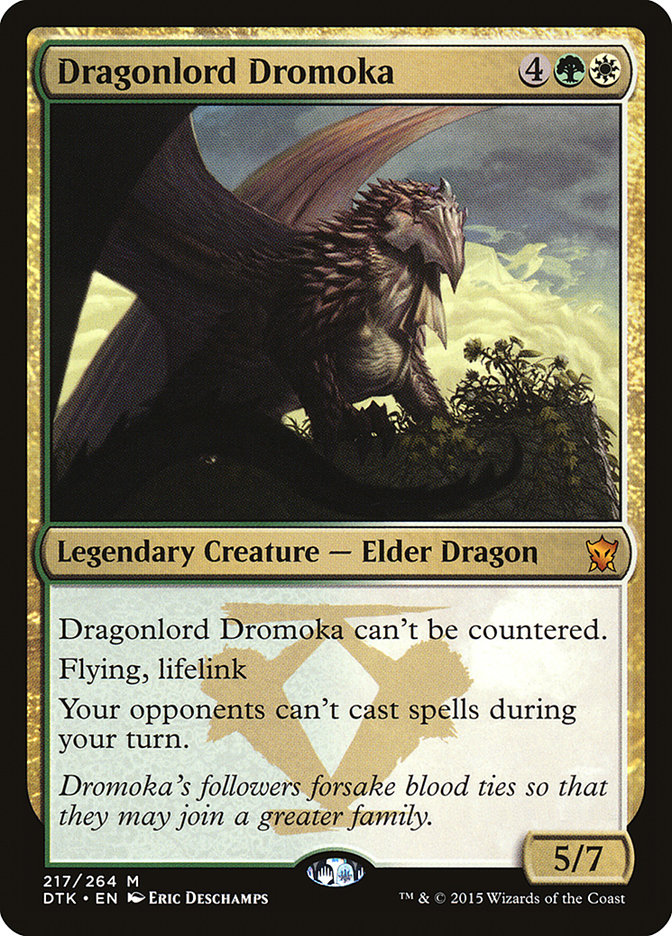
\includegraphics[width=0.9\linewidth]{Cards/dromoka.jpg}
\end{wrapfigure}

Post board we just try to turn into a tempo deck. We bring in all of our counterspells and the two drops. I also try to aggresively mulligan for a turn two threat. The most important card from them is Dromoka because it shuts down our tempo plan while also making us unable to interact. The only good way we have to beat this is gust so we generally try to hold it. Sometimes they play silence. We basically just can't beat that card unless we draw our negate.

In the past they played cards like thought distortion, which immediately ended the game against us. More modern lists usually don't play that card but if they go back to it we can put Narset's reversal in our board to try to fight it. Another possible sideboard option here is test of talents. I think that it is probably too narrow to put in our sideboard against a deck that I don't really see picking up in popularity significantly, even when it looks to be good into the meta.

\begin{center}
    \begin{tabular}{|l|l|}
        \hline
        In           & Out        \\
        \hline
        3 Dispute    & 4 Impulse  \\
        2 Gust       & 3 Axe      \\
        2 Pyromancer & 1 Prismari \\
        1 Negate     & 1 Phoenix  \\
        1 Pierce     &            \\
        \hline
    \end{tabular}
\end{center}

\subsection{UW/UB Control}

\subsection{Convoke}
This matchup is another one that revolves around ledger shredder. If we have a shredder that gets a few triggers we are in a very good spot unless they have the nuts. You should mulligan aggresively for a shredder or a pyromancer post board. In game one we are basically just trying to set up a big enough board to kill them in one swing, usually involving a big shredder and a few phoenixes coming back. Spell pierce is quite good here as an answer to gleeful that also helps protect our shredder from case.

\begin{wrapfigure}{r}{0.25\textwidth}
    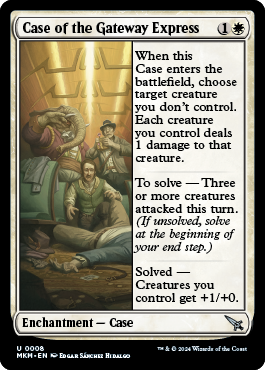
\includegraphics[width=0.9\linewidth]{Cards/case.jpg}
\end{wrapfigure}

I don't have any sweepers in the sideboard because most of them are bad with Jegantha (except cinderclasm which might be worth it if this deck gets more popular). Generally I don't feel like I need them. They are very clunky and line up quite poorly into Thalia and invasion of gobokhan. A pyromancer or shredder that goes unanswered is generally going to do as good of a job at slowing them down.

Since their best cards are gleeful, case, and invasion I like spell pierce. We take out a few of our clunky cards, I'm not entirely sure if I'd rather trim a phoenix or a cruise against them. If you draw multiple of either without a way to set them up it's usually lights out because they are so fast. For now I prefer trimming phoenix because we are bringing in the pyromancers which play much better with cruise than phoenix.

\begin{center}
    \begin{tabular}{|l|l|}
        \hline
        In           & Out        \\
        \hline
        2 Pyromancer & 1 Prismari \\
        1 Pierce     & 1 Phoenix  \\
                     & 1 Proft    \\
        \hline
    \end{tabular}
\end{center}

\subsection{Red Aggro}

\subsection{Niv/Enigmatic}

\subsection{RB Sac}

\subsection{Jund/GB Food}
I think this deck will be more popular than RB sac, but I our plan is basically the same with the only change being that gust is suddenly a very good card. I haven't played against them a ton but it seems to play very similarly, we mainly just need to now be careful to not get Ygra'd rather than get deviled.

\begin{wrapfigure}{r}{0.25\textwidth}
    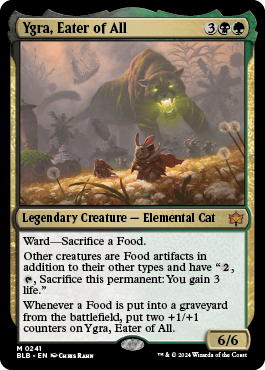
\includegraphics[width=0.9\linewidth]{Cards/ygra.jpg}
\end{wrapfigure}

I think there is a good chance that we want pierce here but I am not fully convinced because most of the cards we care about are very cheap or instant speed. Whether or not we want it may depend on what their sideboard plans end up looking like once the deck is more fully fleshed out. For now I have proft in that spot. I don't think torch is where we want to be because it's not realistically going to get a chance to exile a cat unless the game is already in a spot where we are going to win.

Against the jund deck with fable I think that we could also maybe board in spell pierce since they have fable too. I think that I won't board in the fourth prismari in that spot. It's possible that the fourth prismari isn't even needed against GB, although it gets a lot better if they have hearse in addition to oven. The jund version also has mayhem devil, making it more difficult to lean on prismari as our removal spell. For this reason I leave in three axe in exchange for one of the prismaris not coming in.


\begin{center}
    \begin{minipage}[t]{0.35\linewidth}
        \begin{center}
            \begin{tabular}{|l|l|}
                \multicolumn{2}{c}{\textbf{Standard GB Food}} \\
                \hline
                In         & Out                              \\
                \hline
                3 Prismari & 4 Impulse                        \\
                2 Gust     & 2 Axe                            \\
                1 Proft    &                                  \\
                \hline
            \end{tabular}
        \end{center}
    \end{minipage}
    \quad
    \begin{minipage}[t]{0.35\linewidth}
        \begin{center}
            \begin{tabular}{|l|l|}
                \multicolumn{2}{c}{\textbf{Jund Food}} \\
                \hline
                In         & Out                       \\
                \hline
                2 Prismari & 4 Impulse                 \\
                2 Gust     & 1 Axe                     \\
                1 Proft    &                           \\
                \hline
            \end{tabular}
        \end{center}
    \end{minipage}
\end{center}


\subsection{Waste Not}

\subsection{Spirits}

\subsection{Humans}

\subsection{Ensoul}

\subsection{GW Company}

\subsection{Angels}

\end{document}